\chapter{Test Journal: IMU Variances Test} \label{app:IMUVariances}

\textbf{Date: 06/04/2017}

\subsubsection*{Purpose}
Find the variance of the accelerometer and the variance and bias of the gyroscope present in the IMU, as well as the variance when calculation the attitude using the accelerometer and the magnetometer as described in \autoref{sec:attFusion} in \autoref{eq:roll_acc}, \ref{eq:roll_acc} and \ref{eq:yaw_mag}.

\subsection*{Equipment}
\begin{itemize}
    \item Vessel with all its components.
    %	\item Emlid Reach RTK GPS
    %	\item 2x INLINE 750 14.8V brushless DC-Motor
    %	\item 2x Speed Controller +70 G3.5
    %	\item ADIS16405BMLZ IMU
    %	\item Ps3 Controller  
    \item External laptop.
\end{itemize}

\subsection*{Procedure}
\begin{enumerate}
    \item Turn on all equipment.
    \item Remotely log into the boat, when both, laptop and vessel's computer, are in the same network.
    \item Run the following nodes
    \begin{itemize}
        \item \lstinline[style=cinline]{/lli_node}
        \item \lstinline[style=cinline]{/sensor_node}
    \end{itemize}
    \item Leave the vessel in a fixed position and orientation.
    \item Record the following topics
    \begin{itemize}
        \item \lstinline[style=cinline]{/imu}      
    \end{itemize}
    \item Stop the recording after some time has passed.
    \item Turn off the equipment.
    \item Process the data.
\end{enumerate}

\subsubsection*{Results}

\subsubsection{Accelerometer}
\begin{figure}[H]
    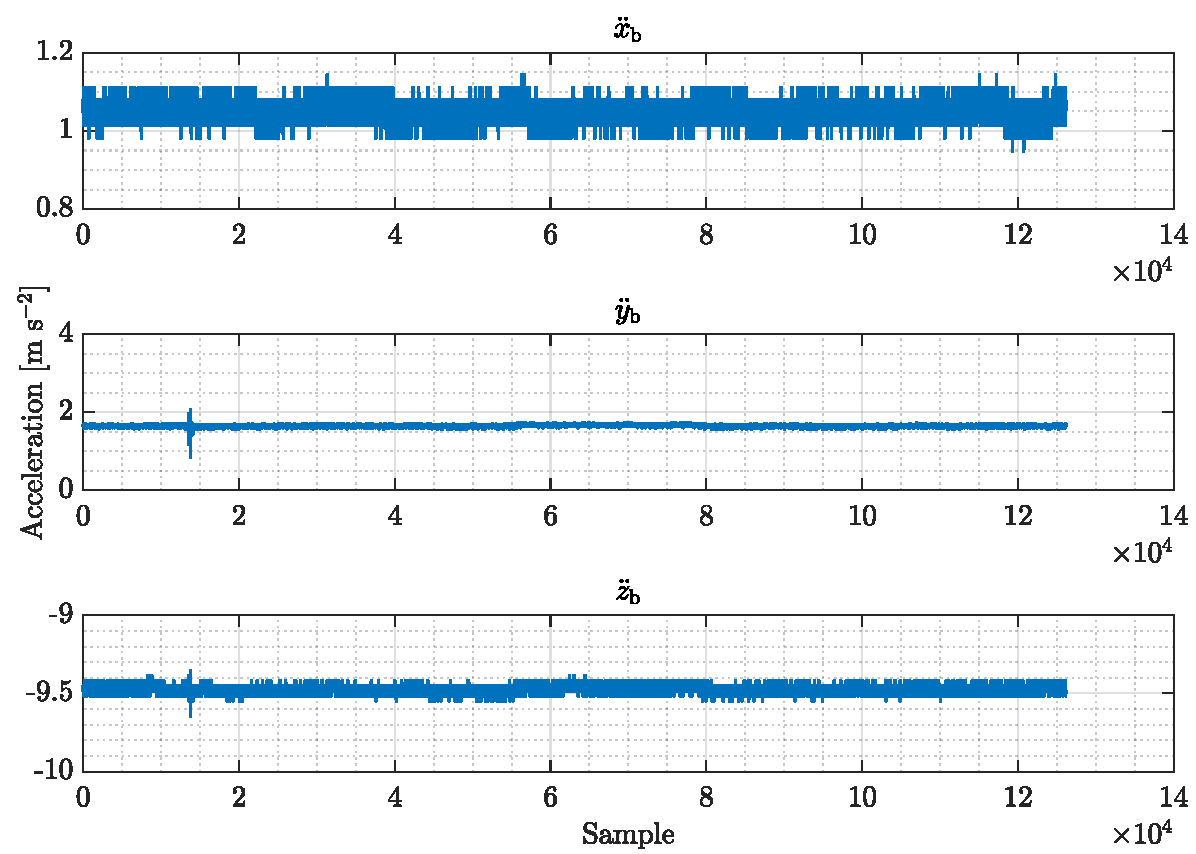
\includegraphics[width=.7\textwidth]{figures/IMUVariancesAcc}
\end{figure}
%
\begin{flalign}
    \sigma_{\ddot{x}\mathrm{b,acc}}^2 & = 0.00050346 \ \mathrm{m}^2 \mathrm{s}^{-4} \nonumber \\
    \sigma_{\dot{y}\mathrm{b,acc}}^2 & = 0.00057036 \ \mathrm{m}^2 \mathrm{s}^{-4} \nonumber \\
    \sigma_{\dot{z}\mathrm{b,acc}}^2 & = 0.00043887  \ \mathrm{m}^2 \mathrm{s}^{-4} \nonumber
\end{flalign}

\subsubsection{Gyroscope}
\begin{figure}[H]
    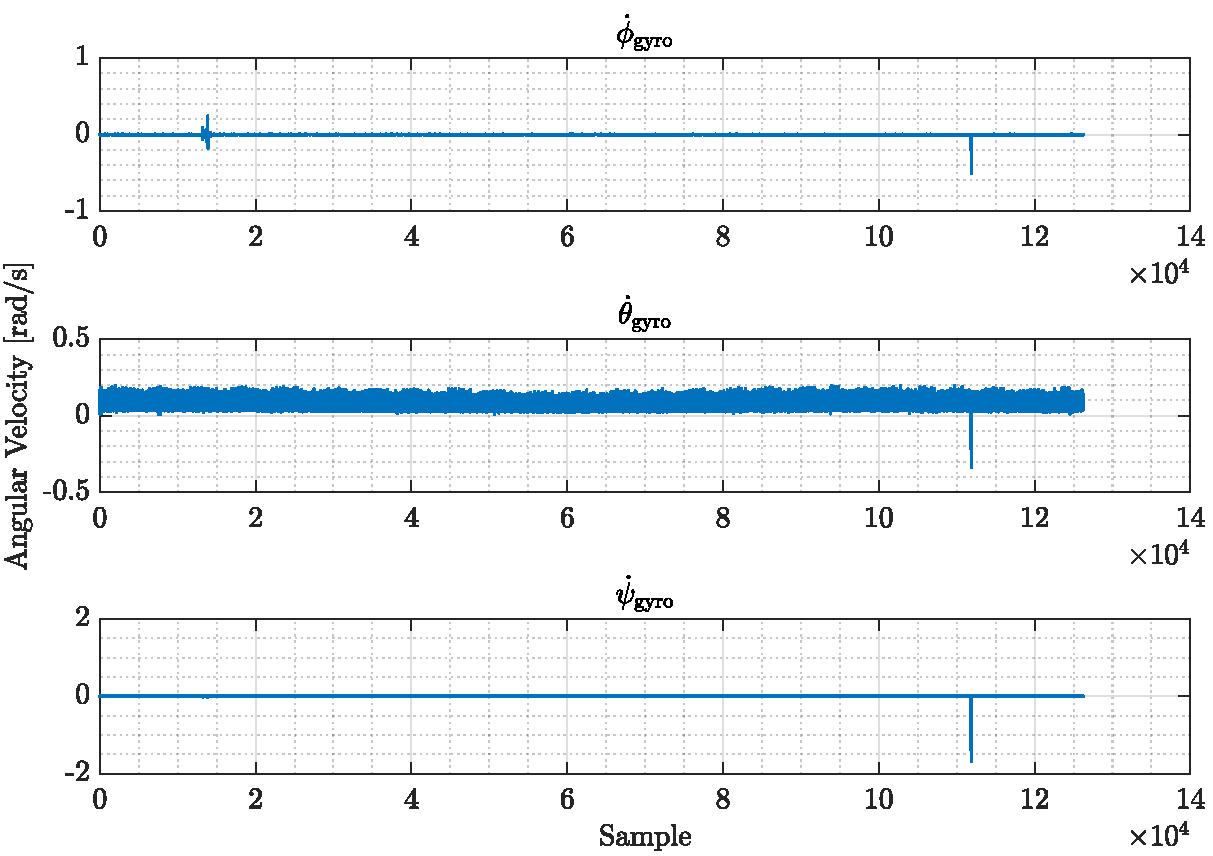
\includegraphics[width=.7\textwidth]{figures/IMUVariancesGyro}
\end{figure}
%
\begin{flalign}
     \sigma_{\dot{\phi}\mathrm{,gyro}}^2 & = 0.01033425 \ \mathrm{rad}^2 \mathrm{s}^{-2} \nonumber \\
     \sigma_{\dot{\theta}\mathrm{,gyro}}^2 & = 3.98414543 \ \mathrm{rad}^2 \mathrm{s}^{-2} \nonumber \\
     \sigma_{\dot{\psi}\mathrm{,gyro}}^2 & = 0.03143791  \ \mathrm{rad}^2 \mathrm{s}^{-2} \nonumber
\end{flalign}
%
\begin{flalign}
    \mathrm{bias}_{\dot{\phi}\mathrm{,gyro}} & = -0.03753465 \ \mathrm{rad s}^{-1} \nonumber \\
    \mathrm{bias}_{\dot{\theta}\mathrm{,gyro}} & = 4.49591086 \ \mathrm{rad s}^{-1} \nonumber \\
    \mathrm{bias}_{\dot{\psi}\mathrm{,gyro}} & = -0.16184524  \ \mathrm{rad s}^{-1} \nonumber
\end{flalign}

\subsubsection{Attitude Calculation}
\begin{figure}[H] 
    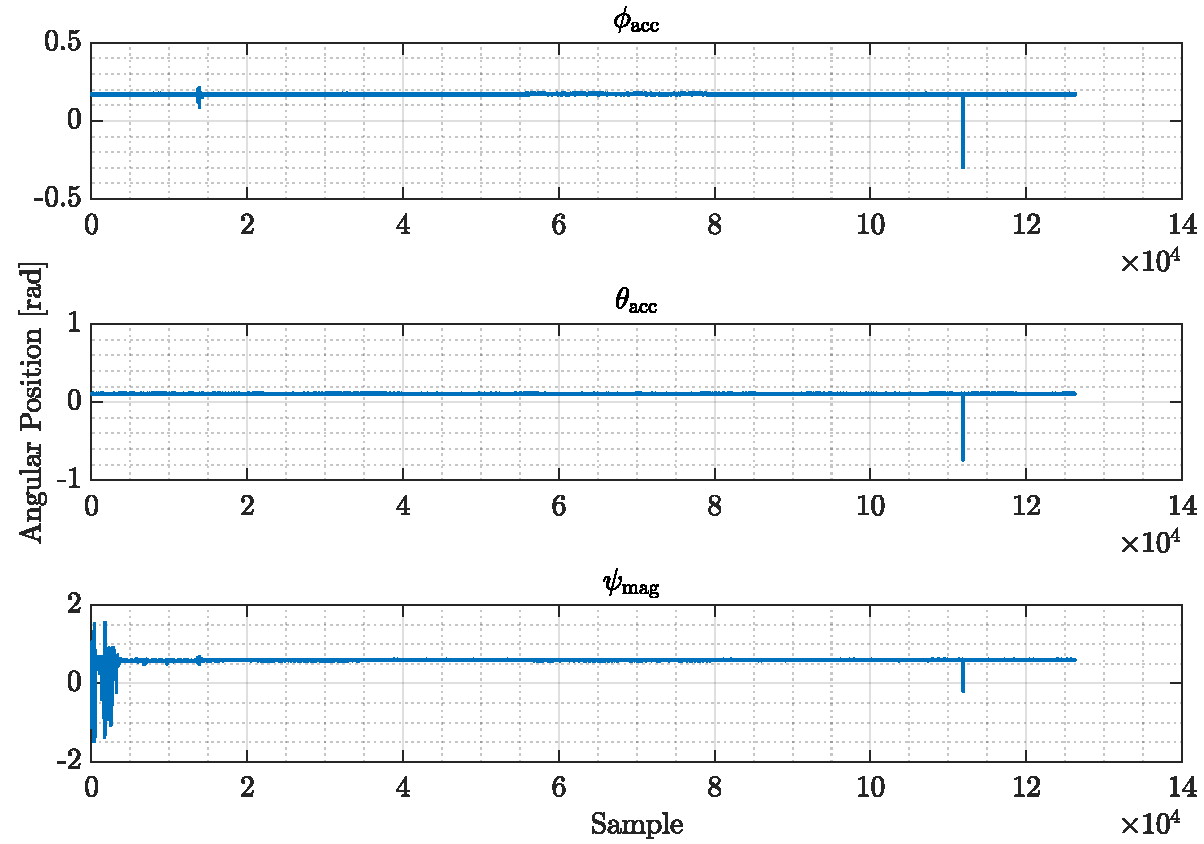
\includegraphics[width=.7\textwidth]{figures/IMUVariancesAtt}
\end{figure}
%
\begin{flalign}
    \sigma_{\phi\mathrm{,acc}}^2 & = 0.00001165 \ \mathrm{rad}^2 \nonumber \\
    \sigma_{\theta\mathrm{,acc}}^2 & = 0.00002264 \ \mathrm{rad}^2\nonumber \\
    \sigma_{\psi\mathrm{,mag}}^2 & = 0.00779021 \ \mathrm{rad}^2 \nonumber
\end{flalign}
